% This is samplepaper.tex, a sample chapter demonstrating the
% LLNCS macro package for Springer Computer Science proceedings;
% Version 2.20 of 2017/10/04
%
\documentclass{llncs}
%
\usepackage{graphicx}

\begin{document}
% Adicionado para por apenas os numeros sem headers
\pagestyle{myheadings}
\title{Development of text-mining solutions to facilitate lipid metabolism interpretation in Genome-Scale Metabolic Models}

\author{Adriano Silva\inst{1}\and
João Ribeiro\inst{1}\and
Emanuel Cunha\inst{1}}

\institute{University of Minho}
%
\maketitle              % typeset the header of the contribution
%
\begin{abstract}
The abstract should briefly summarize the contents of the paper in
15--250 words.

\keywords{First keyword  \and Second keyword \and Another keyword.}
\end{abstract}
%
%
%
\section{Introduction}
\subsection{Context and motivation}
In the past two decades, Systems Biology has emerged as a discipline capable of integrating molecular biological knowledge into an understanding at a system level, from a complete, precise, and efficient perspective.
Biological systems represent a huge amount of data, with the need to be treated and contextualized where this discipline comes to the aid.  
Whether in the construction of stochiometric models or the reconstruction of genome scale metabolic models (GSM), with means to understand the genomic, biochemical, and physiological knowledge gathered \cite{Zou2018,Tavassoly2018}. 
These approaches can guide to strain optimization and the production of a compound with industrial interest, such as lipidic biofuel produced by optimized yeasts and microalgae \cite{Aung2013}.

Impulsed by the advances and cost-effectiveness in technologies that led to high-throughput biological data (Big Data), Systems Biology, and more precisely the reconstruction of GSM models is gaining importance.
The reconstruction of GSM models is taking advantage of the high-quality data generated to create better simulations and predictions. 
In total, since the reconstruction of the first GSM model in 1999 \cite{Edwards1999}, 6239 GSM models were reconstructed until 2019 \cite{Gu2019}. 
Nonetheless, the pace of reconstruction of GSM models can't keep up with the growth of Big Data. The lack of integration of new data in GSM models is a problem inherent to this growth discrepancy.

Besides the usefulness of these models, their reconstruction is limited due to the lack of biochemical and structural data incorporated.
Complex macromolecules are often represented in their generic version not giving any biochemical and structural information.
Particularly in the case of lipids\cite{Aung2013}, only a small chunk of GSM models reconstructed have defined lipids. 
These models neglect the fact that each subclass is constituted of a countless number of combinations between the different components of the lipid. 
Thus the GSM models in these conditions are not able to capture the integrity of lipid biosynthesis network.
Therefore it is important the integration of such information in lipidic models, for a better interpertability, handling and predictions.

Integration of the structural information can be done by taking advantage of the  \emph{de facto} tools such as SWISS LIPIDS \cite{Aimo2015} and  LIPID MAPS \cite{Sud2007}.
As mentioned above this is important to the reliability of the model allowing credible predictions and flexibility in the management of the model.
This can turn into a major advancement in lipid models with better application in industry, such as in the case of lipidic biofuels.




\subsection{Objective}

The main objetive of this project is to integrate structural data, from \emph{de facto} tools SWISS LIPIDS and LIPID MAPS, into a graph-based database BOIMMG.
For that, it will be done an itegration of the synonyms and abbreviations into a new label using ETL pipelines. 

\section{State of art}
\subsection{Genome Scale Metabolic Models}
The use of computational tools brings to the science new tools to face the challenges in the scientific scope.
Among them are GSM models, a computational tool that conjugate biochemical and genomic data from an organism, with the capacity to do \emph{in silico} predictions of a given organism phenotype in specific environmental and genetic conditions \cite{Rocha2007,Zhou2021}.

Thus these models are key to the contextualization of high throughput data and helpful in many other applications such as metabolic engineering, production of biochemicals and bio-materials, prediction of enzyme functions, or even in the discovery of drug targets\cite{Gu2019,Kim2017}.
It is therefore important to integrate fresh and reliable biochemical data in the reconstruction of this models to ensure their accuracy and further atualization \cite{Moseley2021,Passi2021}. 


\subsection{Lipid computational representation}

- Generic/structurally defined duality
-- o que é um lipido, como é a sua estrutura
-- importancia dos lipidos
-- importancia de saber as estruturas dos lipidos
-- como são geralmente representados nos modelos, dualidade generica ou estrutural


\subsection{Generic Representation in GSM models}

- Lipid only with the backbone; 
- Name of the backbone;
- Databases cross-references;

\subsection{Structurally defined representation in GSM models}

- Lipid with the whole structure
- Name composed of backbone and side chains
- No databases cross-references

\subsection{Lack in lipid annotation in GSM models}

- Merge the two previous logics
- Show that one is annotated and the other not.
- Possível Resolução
    - integração dos sinonimos e abreviaturas das bases de dados com ETL (podes por uma frase para cada uma delas e um paragrafo sobre ETL)
    Anotação de modelos:
        - match direto
        - decomposição do nome em dois (backbone e side chain) - queries à base de dados

\subsubsection{Sample Heading (Third Level)} Only two levels of
headings should be numbered. Lower level headings remain unnumbered;
they are formatted as run-in headings.

\paragraph{Sample Heading (Fourth Level)}
The contribution should contain no more than four levels of
headings. Table~\ref{tab1} gives a summary of all heading levels.

\begin{table}
\caption{Table captions should be placed above the
tables.}\label{tab1}
\begin{tabular}{|l|l|l|}
\hline
Heading level &  Example & Font size and style\\
\hline
Title (centered) &  {\Large\bfseries Lecture Notes} & 14 point, bold\\
1st-level heading &  {\large\bfseries 1 Introduction} & 12 point, bold\\
2nd-level heading & {\bfseries 2.1 Printing Area} & 10 point, bold\\
3rd-level heading & {\bfseries Run-in Heading in Bold.} Text follows & 10 point, bold\\
4th-level heading & {\itshape Lowest Level Heading.} Text follows & 10 point, italic\\
\hline
\end{tabular}
\end{table}


\noindent Displayed equations are centered and set on a separate
line.
\begin{equation}
x + y = z
\end{equation}
Please try to avoid rasterized images for line-art diagrams and
schemas. Whenever possible, use vector graphics instead (see
Fig.~\ref{fig1}).

\begin{figure}
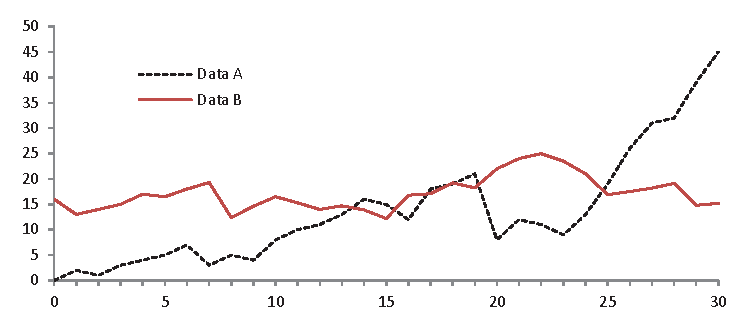
\includegraphics[width=\textwidth]{fig1.eps}
\caption{A figure caption is always placed below the illustration.
Please note that short captions are centered, while long ones are
justified by the macro package automatically.} \label{fig1}
\end{figure}

\begin{theorem}
This is a sample theorem. The run-in heading is set in bold, while
the following text appears in italics. Definitions, lemmas,
propositions, and corollaries are styled the same way.
\end{theorem}
%
% the environments 'definition', 'lemma', 'proposition', 'corollary',
% 'remark', and 'example' are defined in the LLNCS documentclass as well.
%
\begin{proof}
Proofs, examples, and remarks have the initial word in italics,
while the following text appears in normal font.
\end{proof}
For citations of references, we prefer the use of square brackets
and consecutive numbers. Citations using labels or the author/year
convention are also acceptable. The following bibliography provides
a sample reference list with entries for journal


\bibliographystyle{ieeetr}
\bibliography{referencias.bib}
\end{document}
